\documentclass[twocolumn,a4paper,10pt]{article}
\usepackage{graphicx}
\author{DongWei Zhou}
\title{GPSA:A Graph Processing System with Actors}
\begin{document}
\maketitle
\section{Abstract}
Graph-based applications become more and more common due to the rising of the social-networks and other problems come up such as paths of disease outbreaks, or chemical compounds, or biological structures. A strong desire to process large graph motivates researchers to study on distribute memory machines. However, distributed approaches still requires some cost. This cost contains both the access of the distributed resource and the rich experiences for the developers. \newline
While manufacturing technology improves, physical limits of semiconductor-based microelectronics have become a major design concern. A combination of increased available space and the demand for increased thread level parallelism led to the development of multi-core CPUs. Today, a single multi-core server already has a very powerful computing capabilities, which means we can exploit its capabilities to do more job.\newline
In this paper, we present GPSA, a graph processing system with actors on a single machine. In GPSA, we improved the BSP computation model for graph processing according to the feature of the actors. With the new computation model, GPSA could fully exploit the advantage of  multi-core. As a single machine approach, frequent I/O would be an overhead, GPSA utilize the memory mapping for better performance. We show, through experiments and theoretical analysis, that processing large-scale graph on a modern PC with actors performs well.

\section{Introduction}
Graph algorithms are becoming increasingly important for solving many problems in scientific computing, data mining and other domains such as social networks, web graphs, chemical compounds, and biological structures. The scale of real graphs is so large that may consist of billions of vertices, trillions of edges. However, Graph processing is difficult because of the inherent complicated data structure of the graph and the extremely large size of the graph. Therefore, designing a scalable, fault-tolerant, robust system for processing the large-scale graphs is one of the most urgent problems facing systems researchers.\newline
Motivated by the demands, there are already some solutions, which are able to process large scale graphs with distributed system such as Pregle, PowerGraph and GPS, proposed by other researchers. Nowadays, though distributed computional resources are more accessible than ever before, processing these graphs still remains many challenges. In distributed system, the first main problem is workload balancing which caused by partitioning the large scale graph into small partition to fit the cluster nodes. The second main issue is message passing. Messages exit among the different computional nodes or inside of the cluster node, the cluster nodes take cost to communicate with each other and the communication between nodes causes latency which matters in a BSP based graph processing system. Therefore, many researchers spend a lot of energy to study the distributed system based on Pregel to solve the problems mentioned above and some gain reasonable performance, such as Mizan which aims to the workload balancing, GPS focus on the messaging latency. But from a developer’s perspective, developing, debugging and optimizing distributed algorithm on distributed system is quite difficult because the user needs to be skilled at managing and tuning a distributed system in a cluster, which is a nontrivial job for the ordinary user. Besides, these distributed systems need many machines in a cluster which brings both money and energy cost.  \newline
Recently, some graph processing engines on single PC have been proposed to address the problems of the distributed graph systems. Graphchi, a disk-based graph processing engine on a single modern PC, significantly outperforms all representative distributed graph engines.  With complicated design and compute model, these system achieved impressive performance. However, these systems make greate effort to optimize the I/O processing. In GraphChi, the random access problem caused by the locality of the graph urges the GraphChi to propose the disk-based graph computation model. TurboGraph, inspired by GraphChi, focuses on parallelism and overlapping of CPU processing and I/O processing with a novel concept pin-and-slide.  However, neither of them give a fully parallelism computation model for the graph processing which could fully make use of the multicore advantage upon the computation model.
 \newline
Parallelism improves the computing efficiency on the multicore machines. Given the success of parallel computing in scientific computing, data analysis and other areas, parallel processing appears to be necessary to overcome the resource limitations of single processors in graph computations. While the inherent complicated characteristics of the graphs make them hard to match the current parallelism computational problem-solving approaches. Vertex-centric is very brilliant  programming model for the graph processing which proposed by the Pregel. In this mode, every single vertex is a little compute unit, which simplifies the process, and every vertex communicate with each other by message. When a vertex receive a message, the vertex will be actived. If a vertex has no further work to do, the vertex will vote to inactive. 
\newline


 Inspired by the vertex-centric  BSP computation model and parallelism , we present a totally different graph processing engine on a single modern PC. We foucus on how to ultilize the capability of the multi-core and based on that we first improve the BSP model into a parallism computation model with actors. We are bold attempt to assign vertices to actors and transfer the communications among vertices into that of ultra-lightweight actors . In the new model, we decopuled the update function and the message sending function to preocess parallelly which is processed sequential in the traditional BSP model.
 Besides, we notice that the frequent IO processing may be an overhead , we exploit the ability of memory mapping provided by the operating system to gain better performance and simplify the update function.\newline
The rest of the paper is as follows. Section 2 reviews related work. In next section, we will briefly introduce the actor model we used and how we  adopt the vertex-centric model to fit the actor model and show the difference. Section 4 presents the detailed implementation of the system. Section 5 describes the experiments results. And in section 6, and section 7 summarizes and concludes the paper.

\section{Related Work}
Many scalable graph systems have recently been proposed. We survey some of the most relevant works, which may be broadly classified into single-machine approaches and distributed approaches depending on the size of the system.
\newline
Distributed Systems: Pregel is a synchronous vertex-centric programming model proposed by Google for graph system. In Pregel, each vertex is executed in parallel and the user rewrite the compute function invoked by the vertex. Pregel introduced the first bulk synchronous parallel (BSP) distributed message-passing system. In BSP model, all vertex kernels run simultaneously in a sequence of super-steps. Within a super-step, each vertex receives messages from in-neighbor of the last super-step and sends messages to out-neighbor of the next super-step. And a barrier is imposed between two super-steps to guarantee that all vertices finish processing messages.However, Pregel is not open-source and many other systems drown from Pregel such as GPS, PowerGraph, GraphLab, Mizan etc. Other systems Pegasus and gbase are based on MapReduce and support matrix-vector multiplication using compressed matrices.
\newline
Single-machine Systems:X-Stream is a system for processing both in-memory and out-of-core graphs on a single shared-memory machine. X-Stream take advantage of using an edge-centric model and streaming completely unordered edge lists rather than performing random access.  Ligra is a lightweight graph processing framework this is specific for shared-memory multi-core machine. Graphchi is a disk-based single-machine system following the asynchronous vertex-centric programming model. Graphchi proposed parallel sliding windows (PSW) to handling disk-based large-scale graphs and it updates values to the edges in Graphchi. PSW partitions the vertices into P execution intervals, and each execution interval contains a shard file that stores all in-edges sorted by their source vertices. PSW processes one shard at a time. During the processing, first of all, loading an execution interval into memory from the disk, then update the vertices and edges. At last, writing the updated content to disk.

\section{Overview}
While manufacturing technology improves, reducing the size of individual gates, physical limits of semiconductor-based microelectronics have become a major design concern.A combination of increased available space (due to refined manufacturing processes) and the demand for increased thread level parallelism (TLP) led to the development of multi-core CPUs. Since the multi-core has already become the main architecture of the modern PC, in theory, the modern PC should have a powerful computional ability. However, the concurrent computing is still not mature which causes underutilization of the multi-core machines. There are main two ways to implement concurrent computing, multi-process and multi-thread. However, in a single machine, the number of process or thread has its limitation which means poor concurrency and concurrent with thread invoke locks and synchronous. In fact, there is another concept called actor.
\newline
The actor model is a different way of modeling concurrent processes. Rather than threads interacting via shared memory with locks, the actor model leverages "actors" that pass asynchronous messages using mailboxes. A mailbox, in this case, is just like one in real life — messages can be stored and retrieved for processing by other actors. Rather than sharing variables in memory, the mailbox effectively separates distinct processes from each other. Actors act as separate and distinct entities that don't share memory for communication. In fact, actors can only communicate via mailboxes. There are no locks and synchronized blocks in the actor model, so the issues that arise from them — like deadlocks and the nefarious lost-update problem — aren't a problem. What's more, actors are intended to work concurrently and not in some sequenced manner. As such, actors are much safer (locks and synchronization aren't necessary) and the actor model itself handles coordination issues. In essence, the actor model makes concurrent programming easier. The actor model facilitates concurrent programming by allowing a safer mechanism for message-passing. Implementations of this model vary between languages and frameworks. Luckily, there are a number of choices for leveraging this model on the Java platform.

\subsection{Actor of Kilim}
Kilim is a library written in Java that embodies the actor model. In Kilim, "actors" are represented by Kilim's Task type. Tasks are lightweight threads and they communicate with other Tasks via Kilim's Mailbox type. Mailboxes can accept "messages" of any type. Tasks can send String messages or even custom message types — it's entirely up to you. Everything is tied together in Kilim via method signatures; if you need to do something concurrently, you specify the behavior in a method by augmenting its signature to throw Pausable. Thus, creating concurrent classes in Kilim is as easy as implementing Runnable or extending Thread in Java. At last, Kilim's magic is enabled by a post process, called a weaver, which alters the byte code of classes. Methods containing the Pausable throws clause are processed at runtime by a scheduler, which is part of the Kilim library. The scheduler manipulates a limited number of Kernel threads. It is able to leverage this pool for a higher number of lightweight threads, which can context-switch and start up quite fast. Each thread's stack is automatically managed. The actor model makes it easier and safer to write asynchronous-acting objects that depend on similar objects.

\subsection{Model of Computation with Kilim}

 As mentioned above, The vertex-centric programming model introduced by Pregel is based on the Bulk Synchronous Parallel (BSP) computation model. BSP consists of a sequence of super-steps and a barrier is imposed between two super-steps. Within super-step, all vertices kernels run simultaneously. Receiving messages from the last super-step, invoking the user defined computing method, updating the value of the vertices and sending messages to the next super-step. While in a actor, there are no super-steps in conceptually, there is a biggest common thing that both of them involved: message passing. \newline
To implement a BSP model with actor is quite smoothly, because the similarity of vertex-centric programming model and actors. Image that each vertex is an actor and the communication among vertices,in fact, transferring into the communication among actors, which is a very nature thing. However, BSP seems to be more suitable for distributed system because it is simple to implement and allows maximum level of parallelism without the concern of shortage of memory resource during the computation. Besides, every vertex kernel cannot execute simultaneously because of the size of memory and the number of cores of the CPU on a single PC. So does the actors. So even it is the most nature way to implements a BSP model, however, on a single PC is still a challenge. \newline
Here is our BSP computation model with actors that drawn from Vertex-centric and BSP model: From the perspective of actors, vertices are the data carriers and the actors are the basic computational unit and all the message passing among vertices via actors. Instead of storing the messages or combining messages for the next superstep, the worker actors consume the messages immediately once the actors receive the messages. By that way, there is a little different from the traditional BSP model. When an actor need to send a message, it does not have to wait for the computation of the current iteration to finish and send the messages directly because the computation for the current iteration has already been finished in the last iteration.
In our model, we arrange our actors in hierarchy. At the bottom is the dispatcher worker actors and the main computational unit worker. While upon the worker actors is the manager actors who is responsible for global coordinating and monitoring .\newline

\begin{figure}[htbp]
\centering
 \begin{minipage}[]{1.4\textwidth}
     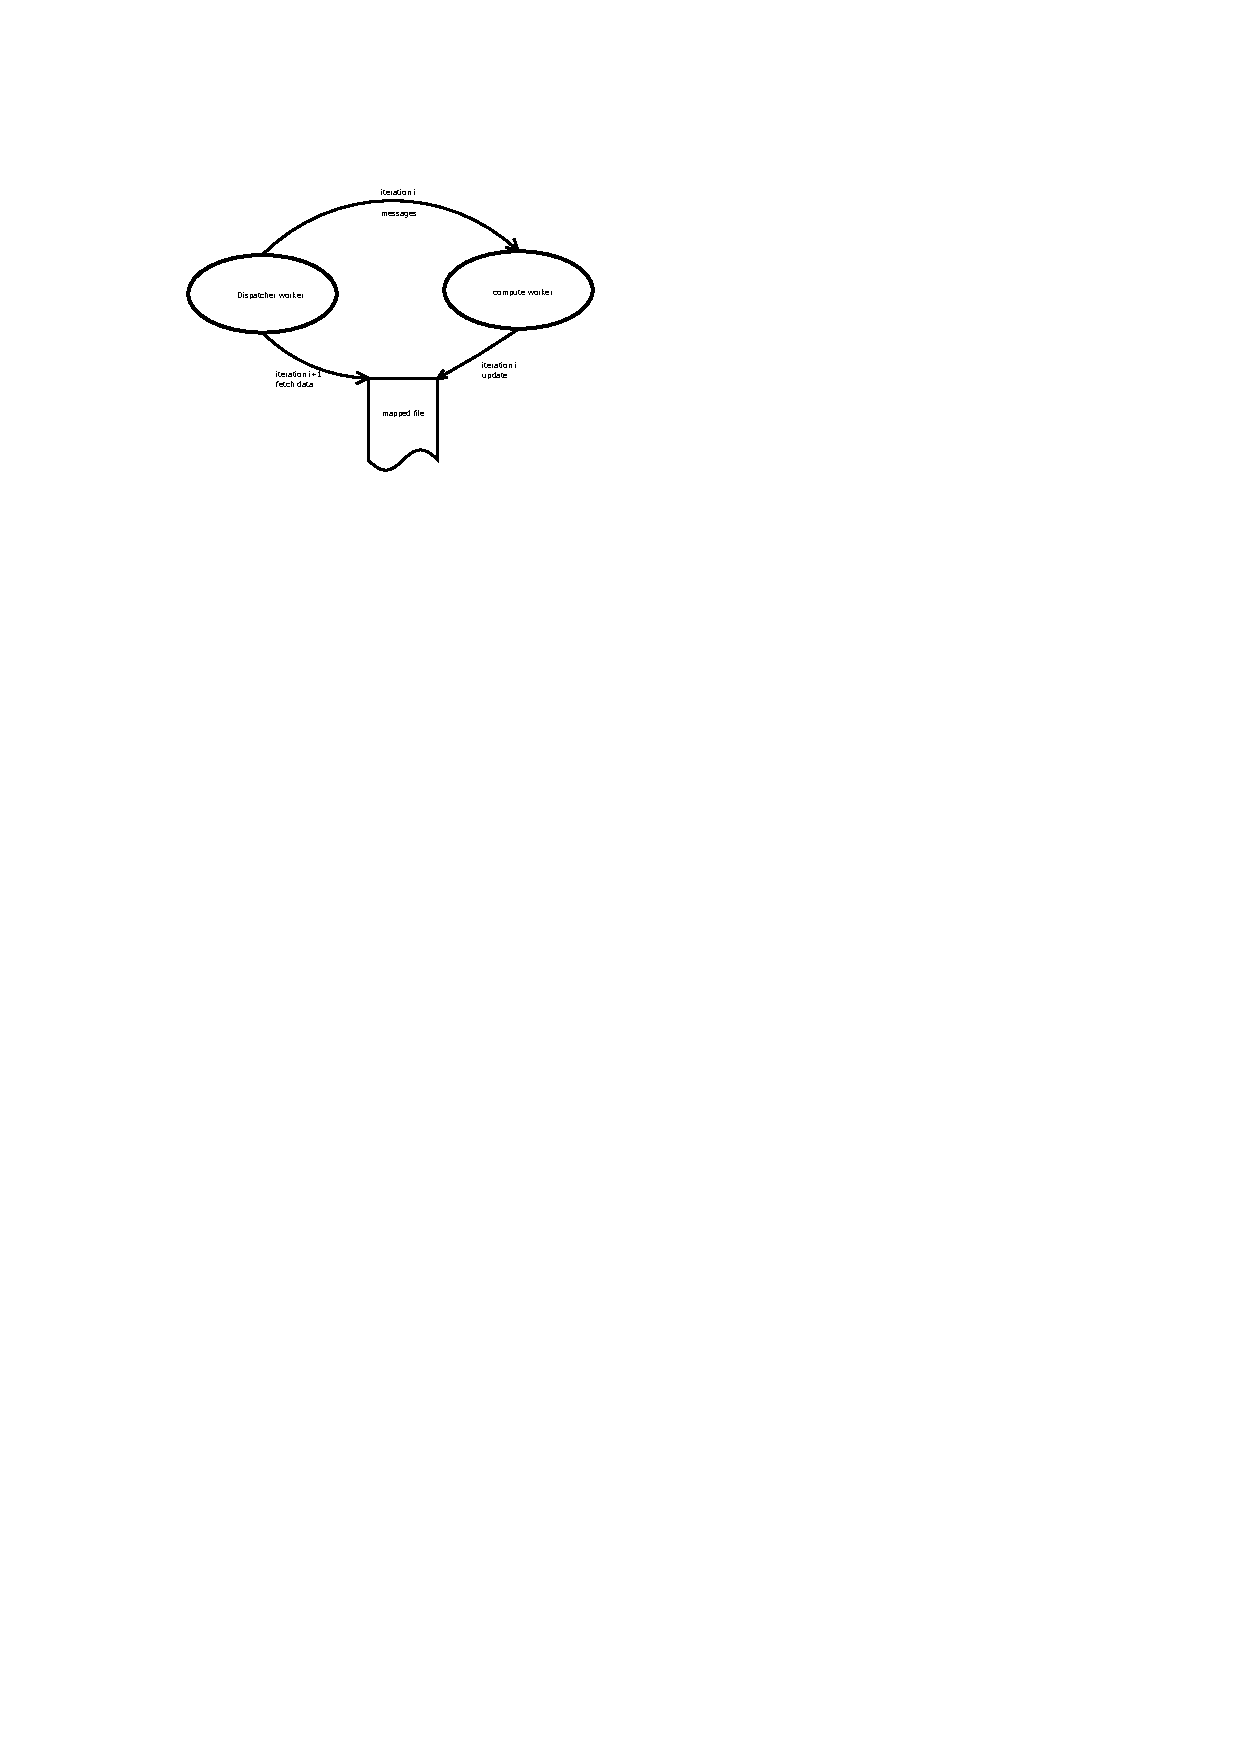
\includegraphics[width=0.4\textwidth,angle=0]{figure/computemodel.pdf}
\end{minipage}
    \caption{compute model with actors}
\end{figure}

We choose the actor model for the graph computation purpose for some reasons. First, the very common nature between vertices and actor makes us to implement the system in a more specific and efficient way by decoupling the computing procedure with the message sending procedure . Second, context switch among actors is more light than that among threads, with actors we could gain quite good performance. there is a great flexibility to implement the model in synchronous or asynchronous way.\newline


\subsection{Synchronous and Asynchronous }
Asynchronous computation model has been studied by many researchers. Asynchronous computation model means that all the vertices subsequently participate in the computation could be able to use the most recently values. The main difference between synchronous and asynchronous is the way of update vertex values. In synchronous implementaion, the value for sending messages in current iteration cannot be modified and update the new value next to the old value. While in asynchronous computation model, the vertex value will be update directly, e.g. the old value will be coverd by the new value which returned by the developer supplied compute method.\newline
In the synchronous model,  fault tolerant will be highly supported, while in the asynchronous model, there is no such feature. To understand this, let us briefly introduce some key technologies used in GPSA. 


\subsection{Memory Mapping and Data Arrangment}
Though ,in GPSA, we foucus on how to compute parallelism on BSP computation model with actors. We also consider the data storage arrangment as well. We take vertex as the data carrier and the actors as the compute or dispatch unit. So we need to store the whole graph in a concise and efficient way or it will be the bottleneck of the system. The main problem caused by I/O is the poor utilization of the caphompute resource in the multicore machine which is the main purpose of the TurboGraph. We reconsider this issume from the operation system level. Actually, in a modern operation system, memory mapping is provided. The primary benefit of memory mapping a file is increasing I/O performance, faster file access, especially when used on large files. Memory-mapping is a mechanism that maps a portion of a file, or an entire file on disk to a range of addresses within an application's address space. The application can then access files on disk in the same way it accesses dynamic memory.

\begin{figure}[htbp]
\centering
 \begin{minipage}[]{1.4\textwidth}
     \includegraphics[width=0.4\textwidth,angle=0]{figure/memorymapping.pdf}
\end{minipage}
    \caption{memory mapping}
\end{figure}

In a 32-bit operating systems, memory-mapped files is usually used for high speed disk access. However, due to the limited address space of the 32-bit operating system, memory-mapped file is less likely used for massive virtual memory or for large files. While in a 64-bit operating system, memory-mapped files can map TB or even PB of memory into a process’s address space. Now that the JVM is 64-bit and could runs on 64-bit operation system, the JAVA developer doesn’t need to consider the disk and the memory as being separate things and could combine them with memory-mapped files via the MappedByteBuffer class. With memory-mapping, the process does not need to bother itself about whether the memory is in RAM or on the disk. The operating system takes care of that which is very fast. 

In order to take advantage of the memory mapping provided by the modern operationg system, we store our graph data into Compressed Sparse Row (CSR) format. As the CSR do not provide any mutability. We sperate the vertex value from the graph and store the value in another memory mapping file.  However, the CSR format stores vertices and edges in separate arrays, with the indices into these arrays corresponding to the identifier for the vertex or edge, respectively. The edge array is sorted by the source of each edge, but contains only the targets for the edges. The vertex array stores offsets into the edge array, providing the offset of the first edge outgoing from each vertex. Iteration over the out-edges for the ith vertex in the graph is achieved by visiting edge_array[vertex_array[i]], edge_array[vertex_array[i]+1], ..., edge_array[vertex_array[i+1]].  
So we need to write the CSR data and the indices information into the mapped file. For the sake of saving memory, we change the CSR a bit. We put an sperator symbol at end. As the figure shown, -1 is the sperator symbol. Sometimes we want to figiure out the outdegree of the vertex, we will write the outdegree at first which indicates how many edges there are, as shown in the figure ------placeholer-----.

\begin{figure}[htbp]
\centering
 \begin{minipage}[]{1.4\textwidth}
     \includegraphics[width=0.4\textwidth,angle=0]{figure/csrdataformat.pdf}
\end{minipage}
    \caption{CSR data format}
\end{figure}

Compare to the sophisticated CSR graph format, the arrangement of the vertex value seems quite simple. We just store the value sequentially. However, there are two totally different computation model. In the synchronous model, we will keep two version of the vertex values. These two version of values is stored next to each other like two columns, as shown in the figure ---placeholer---. The vertex value for message sending which comes from the last iteration will not be updated in the current iteration.  While in the asynchronous model , there is no need to store the value in two columns, because the update will happen on the same column. In this way, we can access the value like an array with a bit mathematics calculation.
\begin{figure}[htbp]
\centering
 \begin{minipage}[]{1.4\textwidth}
     \includegraphics[width=0.4\textwidth,angle=0]{figure/csrdataformat.pdf}
\end{minipage}
    \caption{Value storage and access}
\end{figure}


\subsection{Fault tolerant}
Fault tolerant is important to guarantee the reliability of the system, especially for the high-performance demands. For a graph processing system, a fault-tolerant system must keep track of the whole state of the graph. In GPSA, the graph data i stored in unmutable format, so we can achieve fault tolerant purpose easily. As the synchronous model implemented in the system, all the vertex value is stored  in two-column format. In an iteration, there is always a column is unmutable, which ensure that there is always a copy of right result of the last iteration stored. If the system crash in the current iteration, we can recover the system from the latest successfully finished iteration. While in the asynchronous model, there is a different. As the vertex value will be updated for the later process, the failure will be irretrievable. Because we cannot figure out which value is updated among millions of messages. 
Even we have the manager actor monitoring the whole system, statistics these information could be a burden.  So in the asynchronous model, we don not suggest supporting fault tolerant feature. Otherwise, taking a snapshot of the value file after every iteration finished may be a choice which still could bring unnecessary overhead or uncertaion factor. Furthermore, with the hierarchy of the actor model, the system with actor could be quite robust. The main purpose of the actor model is to break down the large task into small tasks. During the processing, if an actor throws an exception, for the performance reason, the manager actor will handle the exception. If the manager actor also have no idea what to do with the exception, then this exception will report to the supervisor manager actor. \newline

\subsection{Message dispatching}
A message consists of message value and the destination vertex id. In some application, the message value is the update value of a vertex, while it related to both the value and the outdegree in other applications like PageRank. Therefore, we ask the developer to implement the details of how to generate a message value according to the vertex value, outdegree and even the edge weight. If a vertex value has been updated in the last iteration, once the dispatcher worker start to process the updated vertex, it will invoke the user supply method to generate the message value. Then the dispatcher pack the value with the integer id into a byte array and locate the compute worker who will process this message according to the destination id. In fact, there is a great chance that the different adjacent out-edges of a vertex will locate the same compute worker. If the message value has nothing to do with the outdegree or the edge weight, it usually has the same value actually. Packing multi-id with a message value into a complex byte array will reduce the number of the message greatly. Otherwise, if the vertex value did not updated, the dispatcher will skip it.

\subsection{Updating}
In GPSA,  the compute worker will listenning the message receivng eveent. A message comes, the compute worker get the message immediately and break the message into little pieces. According the destination id, it seems to be quite simple to get the vertex value from the value mapped file  and update the value quickly with a simple mathematical calculation. However, to ensure the validity of the update function, it may be the most confused and complex part of the whole system. First, in the asynchronouse model, it won't be a problem. The compute worker fetch the vertex value and compute the value with the message value. Updating the value if a new value is returned or not. \newline
However, in a synchronous model, which implementd in the system, two mainly problems occurs. First, as in the sysnchronous model, the value in the mapped file is stored in two column way for each vertex. One column is used for message sending, the other is used for updating. After one iteration,  two columns of values will become different. So if the compute worker fetch value directly, it will get the wrong data because the validate value is stored in the message sending column actually. So there is a need for the compute worker to figure out the first message of a vertex and fetch value from the message sending column then write it into the updating column.  Second, as mentioned in the last section, if a vertex value is not updated, the dispatcher will skip it. Messages come randomly, it is hard to identify whether a value is updated or not. Though the compute worker knows the updating happened, it has no idead what to do with it. In order to share the update information with the dispatcher, we set the highest bit of the value to 1, which is negative. At first, all the value will be set. During the computation, if a value has been updated, the highest bit will be reset to 0 and write the update. Otherwise, if a message is the first message of the vertex, the negative value will be written.


\section{Implementation}

Similar to the GraphChi, we also assume that the vertices are labeled from 1 to |V| but unlike Graphchi, we uses the compressed sparse row storage format to store the graph in a binary mapped file . And an entry of a vertex is separated by a separator symbol. During the processing, each dispatcher worker will read the mapped file to get the out edges to send messages. In fact, there are different ways to read mapped files to manager the load balance among workers. For example, for the sake of convenience, the vertices can be read by the dispatch actors with a simple mod algorithm. For efficient, assigning these vertices to the dispatcher worker by the average edges to ensure that every dispatcher worker send exactly the same messages. At the same time, the value of the vertex is stored in another mapped file. And each value of the vertex are stored in a memory mapped file in ascending order by its label. In this way, we can access the data in a sequential way like a normal array. For example, for a vertex whose id is k, the start index of its value stored in the mapped file could be figure out by the equation index = id * sizeof(value)*factor. 

 When the data has already been mapped into memory, manager tells its workers that data is ready. And the workers will start fetching their data from the file at the certain position, which means they can read data full parallel. Unlike the traditional BSP model, we decouple the compute and the send method. At first, we keep two copies of the initialized values. In an iteration, the worker do mainly two things: dispatching messages and computing messages. Once get the data, the worker start its execution loop. During the loop, worker will dispatch the messages to the destination worker according to the out edges of the fetched data. Once another worker actor receive the message, it will directly compute the message with certain value and put the updated value into memory mapped file. In this way, the update function and send function has no relationship with each other in the current iteration.
//添加计算流程图

\subsection{Manager Actor}
The main responsibility of the manager actor is coordinating the computation, exception handling, worker monitoring. Each manager will keep track of the states of its own workers. When the computation start, the manager will send workers an ITERATION\_START signal and the worker who receive this command will start execution immediately. When a dispatcher worker finish all its dispatching work in current iteration, it will inform the manager with a DISPATCH\_OVER signal. Once all the works send DISPATCH\_OVER signal to its manager, the manager knows time to get into next iteration and send COMPUTE\_OVER signal to its compute workers. After the compute workers receiving this, they will know this is the last message of the current iteration. Then the worker will reply with a COMPUTE\_OVER signal. At the end, an SYSTEM\_OVER signal will kill all the worker actors and finish the job.

\subsection{Worker Actor}
Worker actor is the most important role of the system. They are the basic execution units. There are two kinds of worker, dispatcher worker and compute worker. Dispatchers is responsible for reading edges and send vertex update messages to compute workers. The compute workers listen the message receiving event. If there is a message arrived, the compute worker get the message from its own mailbox and compute the message with user supplied compute() method.
Inside of the dispatchers, the sequence of the vertex id and the interval of the index of the compressed sparse row mapped file are maintained. According to the sequence, the worker actor will clearly know where and how to get next data entry and the associated edges. If the iteration ends and a new iteration starts, the sequence will be reset to start over again. 
The dispatchers is the bridge connected the compute workers with the manager. When the dispatchers has already finished their jobs, the compute workers usually still has a little tails to clean up. So the dispatchers notify the manager that the dispatcher for the current iteration has finished. At this moment, in the system, there is no more messages passing around, then the manager send a compute over message appending the end of the mailbox of each compute worker. When the compute worker get the compute over message, it will aware that there is no more messages to process in the current iteration.

\section{Experiment}
We compare our framework with the GraphChi, a state-of-the-art approache, by measuring the elapsed times of two classic graph algorithms and the useage of the CPUS. We will show how simple it is to implements the algorithm with our system , then we introduce the setup environment and the data sets used for the experiment.And at last, we present and discuss our results. We selected two graphs with different size: a google network with 5 million edges, and a LiveJournal network with 69 million edges. 


\end{document}
